\newif\ifPAPER  
\PAPERtrue % select either slide or note
%\PAPERfalse  

\def\g4{{\sf Geant4}}

\newcommand{\codeAlgorithm}[1]{
\addcontentsline{toc}{section}{Résumé}
\begin{center}\fbox{\parbox{12cm}{\bf #1}}\end{center}}

\newcommand{\cppintro}[1]{
\lstset{language=C,
caption= #1 ,
label=listing:boundary}}

\def\cppstart{\begin{lstlisting}}
\def\cppend{\end{lstlisting}}

\newif\ifCITENOTE 
\CITENOTEtrue

\ifPAPER
\documentclass[twoside,floatfix,a4wide]{d}
\usepackage{multirow}
\usepackage{url}
\usepackage{listings}
\usepackage{graphicx}
\usepackage{wrapfig}
%\usepackage{makeidx}
\usepackage{subfig}
\usepackage{fancyhdr}
%\usepackage{asymptote}
\usepackage{amsmath}
\usepackage{verbatim} % for comment
\usepackage{eurosym} 
\usepackage{color} % for definecolor
\usepackage[colorlinks,bookmarks=true]{hyperref}

\numberwithin{equation}{section} % reguires amsmath-package
\pagestyle{fancy}
\fancyhead{} % clear all fields

\fancyhead[L]{\it {Helsinki, May 4, 2009}} % Left Odd, Right Even 
\fancyfoot[L]{G.Danielsen - Simulating carbon beam fragmentation on water phantom with the Geant4 INCL/ABLA models} 
\fancyhead[R]{\thepage}
\fancyfoot[C]{}
\newcommand{\urltilde}[1]{\texttt{#1}} % solves the tilde problem

\graphicspath{{images/}}
\DeclareGraphicsRule{.eps.gz}{eps}{.eps.bb}{`gunzip -c #1} % zipped images

\definecolor{light-gray}{gray}{0.95}
\definecolor{dark-gray}{gray}{0.30}
\definecolor{orange}{rgb}{1,0.5,0}
\definecolor{dark-blue}{cmyk}{1,0.5,0.5,0}
\hypersetup{
    bookmarks=true,         % show bookmarks bar?
    unicode=false,          % non-Latin characters in Acrobat’s bookmarks
    pdftoolbar=true,        % show Acrobat’s toolbar?
    pdfmenubar=true,        % show Acrobat’s menu?
    pdffitwindow=true,      % page fit to window when opened
    pdftitle={My title},    % title
    pdfauthor={Author},     % author
    pdfsubject={Subject},   % subject of the document
    pdfnewwindow=true,      % links in new window
    pdfkeywords={keywords}, % list of keywords
    colorlinks=true,        % false: boxed links; true: colored links
    linkcolor=dark-blue,          % color of internal links
    citecolor=dark-blue,        % color of links to bibliography
    filecolor=dark-blue,         % color of file links
    urlcolor=dark-blue            % color of external links
}
\begin{document}

\title{Simulating carbon beam fragmentation on water phantom with the Geant4 INCL/ABLA models}


\author{Gillis Danielsen$^1$ mentored by A.~Heikkinen$^2$} 
\affiliation{$^1$ Helsinki University of Technology}
\affiliation{$^2$ Helsinki Institute of Physics, P.O. Box 64, FIN-00014 University of Helsinki (Finland)}
\begin{titlepage}
\pagestyle{empty}
\begin{center}
rev. 001-2009\\
\vspace{7.5 cm}
\Huge
Simulating carbon hhhbeam fragmentation on water phantom with the Geant4 INCL/ABLA models\\

\vspace{5cm}

\Large
Gillis Danielsen, Bachelor's Thesis\\
Helsinki University of Technology\\

    \vspace{0,2cm}
  \end{center}

\end{titlepage}


\begin{abstract}
This work focuses on the simulation of carbon beams in a water phantom using GEANT4 code. Results will be compared to experimental data made available by the GSI Darmstadt/E.Haettner.

\footnote{Bachelor's thesis produced in the framework of the Finnish CERN Summer Training 2009.}
\end{abstract}
\maketitle
\thispagestyle{fancy}

\tableofcontents

\section{Introduction}
\begin{itemize}
\item CERN, CEA and HIP
\item Simulations
\item $C_{12}$ beams in water
\item reference data provided from GSI (E. Haettner, Master's thesis, KTH)
\item applications in Hadron treatment
\item Structure of this report
\end{itemize}
This paper focuses on the simulation of carbon beams in a water phantom using GEANT4 code as a medical application. GEANT4 is a multi-purpose physics simulation package developed at CERN, Switzerland. GEANT4 currently hosts multiple models suitable for the experiment, but this paper will focus on the INCL and ABLA models developed as a collaboration of scientists at CERN, HIP and CEA (tarkenna, nimet).

The history of radiation treatments dates back to the late 19th century when W.K. Roentgen discovered the X-rays. It was not long before these photon rays were being used to treat malign tissue. The first methods used were on today's standards very crude, and much work has gone into perfecting the treatments in order to minimize the effect of the rays on the surrounding healthy tissue and maximize the dose delivered to the malign tissue.

However, due to the statistical nature of the photon interactions, a beam of many photons is
exponentially attenuated yielding an exponential decrease of the dose with the depth. To
obtain a higher dose in the tumor than in the surrounding normal tissue, many irradiation
fields are used. The cost of this method is that a large volume of the normal tissue
will suffer from a high dose. By replacing the x-rays with high energy photons, the dose
maximum is shifted a few centimeters deeper and the exponential decrease is more shallow,
which improves the ratio between dose in the tumors and in the normal tissue.

Although very sophisticated variations of the photon treatments have been perfected over time, photon therapies still produce considerable harm to the surrounding tissue. A much younger and less widely used technology are those of hadron- or heavy-ion based radiotherapies. Hadrons and heavyer-ions are charged particles and therefore react to tissue in a much different way to photons. The dose-profile contains a much sharper peak due to the primary halting force being electromagnetic interaction. This peak is called the bragg-peak, and was first discovered by William Henry Bragg in 1903.

The field of hadron treatments were pioneered by Berkeley. Based on research done at the Berkeley cyclotron J.Wilson first recomended the use of protons as a treatment method in a ... paper and the first de facto treatment was administered at Berkeley in 1953. Today there are is a number of proton-based therapies in clinical use around the world.

Heavy-ion therapies have remained considerably less common and have remained on a more experimental level. Clinical trials were conducted at Lawrence Berkeley Laboratory (LBL) inbetween 1977 and 1993 with $Ne_20$. To date PCTOG estimates that more than 5000 heavy-ion treatments have been made. Treatments based on carbon beams have been offered at NISR in Japan and in Germany at GSI.

The motivations for heavy-ion treatments as an alternative to hadron treatments are considerable as carbon ions have an added advantage of higher ionisation-density at the end of their range, this will cause greater correlated damage to the DNA-structure of a single cancerous cell and therefore make it more likely that cell is unable to repair. The papers ... approximate the beam's increase in biological efficiency of the dose by a factor between 1.5 and 3 in comparison to proton treatment. Heavy-ions ions are also less scattered in lateral directions which yields better control in many applications. However, as a tradeoff carbon-ions will produce smaller particles due to fragmentation, yielding an unwanted ``tail`` to the energy-loss profile.

A number of data-sets are available for carbon beams. This paper will use the beams measured by E. Haettner ~\cite{ehaettner}  at the GSI Darmstadt facilities data comparison, and therefore aims to mimic that experiment setup. The aim of this paper is  to provide good reference data for the standardization work involved in hadron treatments as well as to evaluate the feasibility of the GEANT4 models for such simulations by comparison to experimental data.

\section{Theory}
\begin{equation}
 \frac{dE}{dx} = \frac{4 \pi}{m_e c^2} \cdot \frac{nz^2}{\beta^2} \cdot \left(\frac{e^2}{4\pi\varepsilon_0}\right)^2 \cdot \left[\ln \left(\frac{2m_e c^2 \beta^2}{I \cdot (1-\beta^2)}\right) - \beta^2\right]
\label{bethebloch}
\end{equation}


\begin{itemize}
 \item E. Haettner
 \item ABLA documentation
\end{itemize}
\begin{figure}
\begin{center}
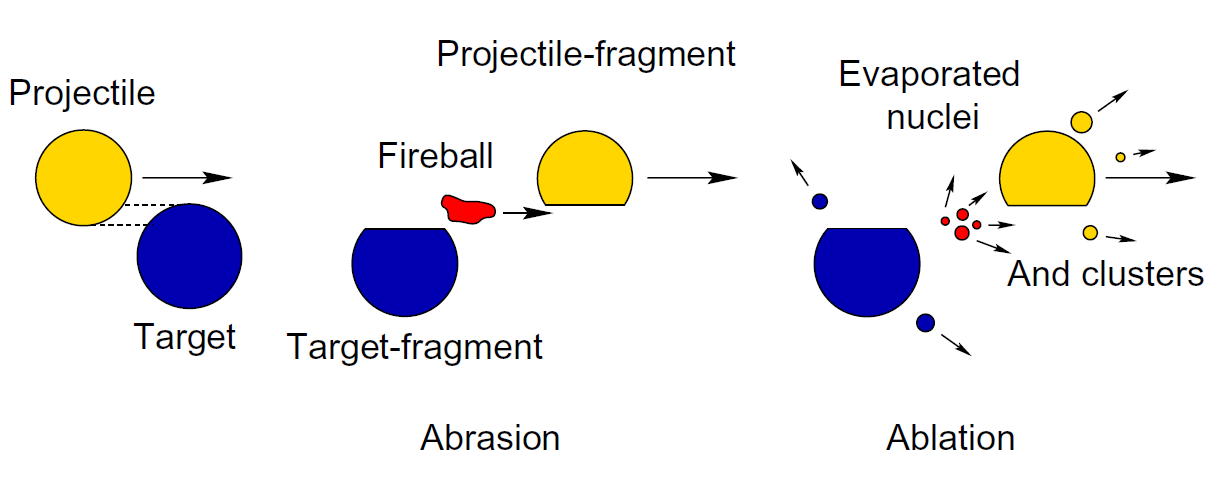
\includegraphics[width=0.8\textwidth]{images/ablationabration.png}  
\caption{Schematic of the physics involved.}
 \label{fig:ablationabration}
 \end{center}
 \end{figure}
\begin{figure} 
\begin{center}
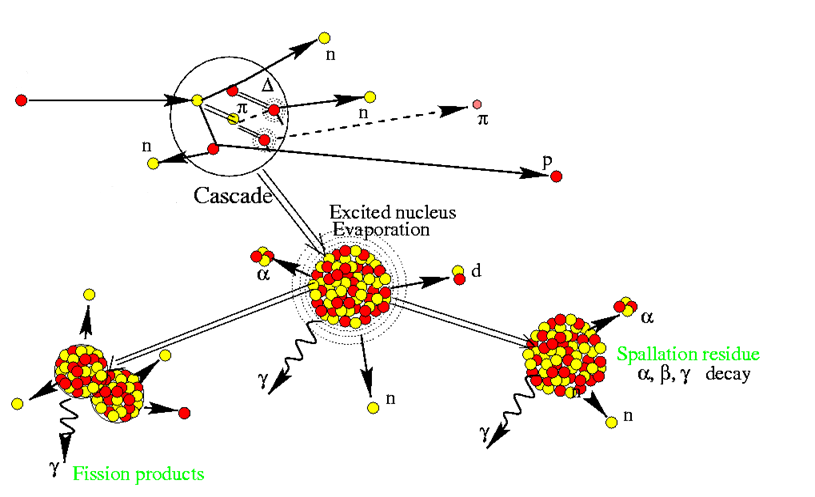
\includegraphics[width=0.8\textwidth]{images/inclScematic.png}  
\caption{\label{fig:inclschematic} Schematic diagram of INCL and ABLA models.}
 
 \end{center}
 \end{figure}


\section{Simulation setup}
\begin{itemize}
\item Experiment data from GSI
\item target description
\item Characterization of the beam
\item Simulation of detectors
\item Implementation details
\end{itemize}

\section{Results and comparison to GSI data}
\begin{itemize}
\item comparison (Haettner 5.4.1)
\item energy distribution of fragments
\end{itemize}

\section{Conclusion}
\begin{itemize}
\item Raflaava yhteenveto
\end{itemize}

\section{Appendices}
\begin{itemize}
\item code examples
\item runtime log
\end{itemize}





\bibliographystyle{plain} \bibliography{refs.bib} 
\end{document}

\else

\fi